\documentclass[tikz,border=4mm]{standalone}

\usepackage[T1]{fontenc}
\usepackage{amsmath,amssymb,bm}
\usepackage{newtxtext,newtxmath}
\usetikzlibrary{arrows.meta,calc,positioning}

\definecolor{ink}{HTML}{1F2A44}
\definecolor{accent}{HTML}{9A3B2F}
\definecolor{sea}{HTML}{2E6E6B}
\definecolor{sand}{HTML}{F2EEE6}
\definecolor{ash}{HTML}{6B7280}

\newcommand{\xt}{\bm{x}_t}
\newcommand{\zz}{\bm{z}}
\newcommand{\Id}{\bm{I}}
\newcommand{\epsb}{\bm{\epsilon}}

\begin{document}
% Exact figure source from chapters/04-marginal.tex (fig:score-distill).
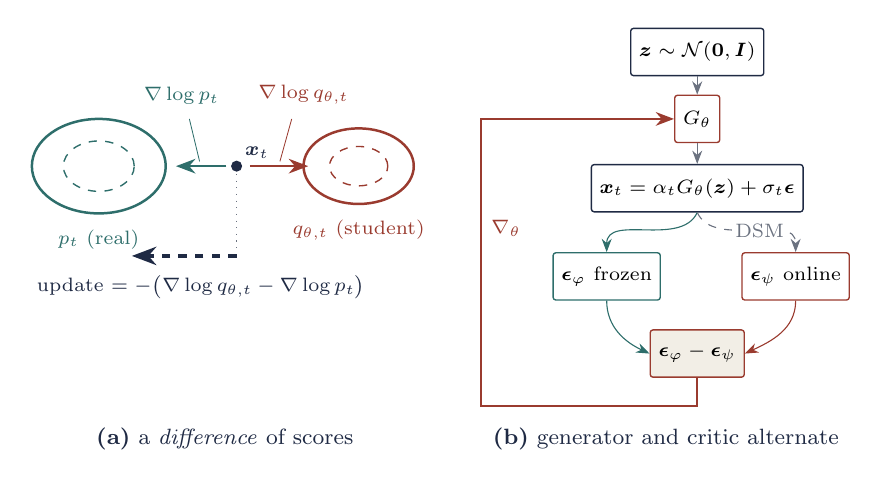
\begin{tikzpicture}[>=Stealth,font=\footnotesize]
% ---------------- panel (a): the two-score gradient
\begin{scope}[yshift=1.25cm]
  \draw[sea,line width=.9pt] (0,0) ellipse (0.85 and 0.60);
  \draw[sea,line width=.5pt,dashed] (0,0) ellipse (0.45 and 0.32);
  \node[color=sea,font=\scriptsize,anchor=north] at (0,-0.68) {$p_t$ (real)};
  \draw[accent,line width=.9pt] (3.3,0) ellipse (0.70 and 0.48);
  \draw[accent,line width=.5pt,dashed] (3.3,0) ellipse (0.37 and 0.25);
  \node[color=accent,font=\scriptsize,anchor=north] at (3.3,-0.56) {$q_{\theta,t}$ (student)};

  \fill[ink] (1.75,0) circle (2pt);
  \node[color=ink,font=\scriptsize,anchor=south west,inner sep=1.5pt] at (1.80,0.04) {$\xt$};
  \draw[sea,->,line width=.9pt]    (1.62,0) -- (0.98,0);
  \draw[accent,->,line width=.9pt] (1.92,0) -- (2.66,0);
  \node[color=sea,font=\scriptsize,anchor=south] at (1.05,0.66) {$\nabla\log p_t$};
  \draw[sea,line width=.3pt] (1.28,0.06) -- (1.15,0.60);
  \node[color=accent,font=\scriptsize,anchor=south] at (2.60,0.66) {$\nabla\log q_{\theta,t}$};
  \draw[accent,line width=.3pt] (2.30,0.06) -- (2.45,0.60);

  \draw[ash,dotted,line width=.4pt] (1.75,-0.10) -- (1.75,-1.06);
  \draw[ink,->,line width=1.3pt,dashed] (1.75,-1.14) -- (0.42,-1.14);
  \node[color=ink,font=\scriptsize,anchor=north,align=center] at (1.30,-1.26)
     {update $=-\bigl(\nabla\log q_{\theta,t}-\nabla\log p_t\bigr)$};
\end{scope}

% ---------------- panel (b): the alternating loop
\begin{scope}[xshift=6.6cm,yshift=0.35cm,
  b/.style={draw=ink,fill=white,rounded corners=1pt,inner sep=3pt,
            minimum height=6mm,line width=.5pt,align=center,font=\scriptsize}]
  \node[b] (z) at (1.0,2.35) {$\zz\sim\mathcal N(\bm0,\Id)$};
  \node[b,draw=accent] (g) at (1.0,1.50) {$G_\theta$};
  \node[b] (noise) at (1.0,0.62) {$\xt=\alpha_t G_\theta(\zz)+\sigma_t\epsb$};
  \node[b,draw=sea] (real) at (-0.15,-0.50) {$\epsb_\varphi$ frozen};
  \node[b,draw=accent] (fake) at (2.25,-0.50) {$\epsb_\psi$ online};
  \node[b,fill=sand,draw=accent] (diff) at (1.0,-1.48) {$\epsb_\varphi-\epsb_\psi$};

  \draw[->,ash] (z) -- (g);
  \draw[->,ash] (g) -- (noise);
  \draw[->,sea]        (noise.south) to[out=-115,in=90] (real.north);
  \draw[->,ash,dashed] (noise.south) to[out=-65,in=90]
      node[pos=.55,color=ash,font=\scriptsize,fill=white,inner sep=1pt] {DSM} (fake.north);
  \draw[->,sea]    (real.south) to[out=-90,in=155] (diff.west);
  \draw[->,accent] (fake.south) to[out=-90,in=25]  (diff.east);
  \draw[->,accent,line width=.8pt]
      (diff.south) -- (1.0,-2.15) -- (-1.75,-2.15) -- (-1.75,1.50)
      node[pos=.62,right,color=accent,font=\scriptsize] {$\nabla_\theta$} -- (g.west);
\end{scope}

\node[color=ink,anchor=north] at (1.60,-1.95) {\textbf{(a)} a \emph{difference} of scores};
\node[color=ink,anchor=north] at (7.20,-1.95) {\textbf{(b)} generator and critic alternate};
\end{tikzpicture}
\end{document}
